\documentclass[
	spanish,
	9pt,
	xcolor=table,
	handout,
	aspectratio=1610,
	%ignorenonframetext
]{beamer}

\usepackage[spanish]{babel}
\usepackage[
	cursointroductorio,
	fullpagenumbering
]{dunestyle-beamer}
%\usepackage{svg}
%\graphicspath{{./images}}
\usepackage{booktabs}
\usepackage{longtable}

\usepackage[backend=biber,style=numeric, defernumbers=true, sorting=ynt,maxbibnames=4,maxcitenames=4]{biblatex}
\addbibresource{dune-webinar-references.bib}

\title{
	Una introducción a la caja de herramientas DUNE en \texttt{C++}/\texttt{Python} para la solución de modelos matemáticos
}
\subtitle{
	Parte I:
	\lstinline{bash}
}

\author{}
\institute[]
{
	\noindent
	Practique los ejemplos en Gitpod

	\href{https://gitpod.io\#/https://github.com/cpp-review-dune/dune-webinar}{
\includegraphics[width=4.5cm]{open-in-gitpod}}

	\vfill

	\begin{minipage}{0.12\paperwidth}
		Disponible en
	\end{minipage}%
	\hfill%
	\begin{minipage}{0.18\paperwidth}
		\href{https://github.com/cpp-review-dune/dune-webinar}{
\includegraphics[width=1.2cm]{GitHub-Mark-120px-plus}}
	\end{minipage}

	\vfill

	\begin{minipage}{0.26\paperwidth}
		¡Únete al grupo en Telegram!
	\end{minipage}%
	\hfill%
	\begin{minipage}{0.04\paperwidth}
		\href{https://t.me/joinchat/OsfYP1xnFlxjN2Ix}{
\includegraphics[width=1.2cm]{telegram-logo}}
	\end{minipage}

}

\setbeamertemplate{bibliography item}{%
	\ifboolexpr{ test {\ifentrytype{book}} or test {\ifentrytype{mvbook}}
		or test {\ifentrytype{collection}} or test {\ifentrytype{mvcollection}}
		or test {\ifentrytype{reference}} or test {\ifentrytype{mvreference}} }
	{\setbeamertemplate{bibliography item}[book]}
	{\ifentrytype{online}
		{\setbeamertemplate{bibliography item}[online]}
		{\setbeamertemplate{bibliography item}[article]}}%
	\usebeamertemplate{bibliography item}}

\defbibenvironment{bibliography}
{\list{}
	{\settowidth{\labelwidth}{\usebeamertemplate{bibliography item}}%
		\setlength{\leftmargin}{\labelwidth}%
		\setlength{\labelsep}{\biblabelsep}%
		\addtolength{\leftmargin}{\labelsep}%
		\setlength{\itemsep}{\bibitemsep}%
		\setlength{\parsep}{\bibparsep}}}
{\endlist}
{\item}

\begin{document}

{
\usebackgroundtemplate{
	\centering
	
\includegraphics[width=\paperwidth]{duneslides-logo}
}
\begin{frame}[plain,noframenumbering]

	\color{c++reviewduneblue}

	\begin{flushleft}\bfseries\scshape\huge
		Una introducción a la caja de herramientas DUNE Numerics
		para la solución de modelos matemáticos
	\end{flushleft}

	\

	\

	\

	\

	\

	\

	%\begin{minipage}{0.47\textwidth}
	%	\begin{figure}[ht!]
	%		\centering
	%		
\includegraphics[height=1.5cm]{alfaomega}
	%		\caption*{
	%			\large
	%			\bfseries
	%			\textcolor{c++reviewduneblue}{Webinar 13 de Julio de 2021}
	%		}
	%	\end{figure}
	%\end{minipage}
	\begin{minipage}{0.5\textwidth}
		\begin{flushright}
			\large
			\bfseries
			Elaborado por:\\
			John Jairo Leal Gómez\\
			Universidad Nacional de Colombia\\
			Carlos Alonso Aznarán Laos\\
			Universidad Nacional de Ingeniería, Perú
		\end{flushright}
	\end{minipage}
	\note{
		En este webinar se presenta en dos partes, por un lado presentaremos el libro: \emph{Las matemáticas en la vida real, introducción básica al modelamiento matemático} y en segundo lugar se hará una presentación de la biblioteca modular DUNE.
	}
\end{frame}
}
\section{Presentación del libro}

\begin{frame}
	\frametitle{\secname}
	\begin{minipage}{0.5\textwidth}
		\begin{figure}[ht!]
			\centering
			\href{https://www.uneditorial.com/las-matematicas-en-la-vida-real-introduccion-basica-el-modelamiento-matematico-matematica.html}{
\includegraphics[height=6.8cm]{portada}}
		\end{figure}
		\note{
			Los autores, John Jairo Leal y Juan Pablo Cardona les
			compartimos nuestro texto, y les contamos que es el producto de
			varios proyectos educativos de modelamiento matemático en las
			aulas en cursos de ingeniería.

			Una de nuestras líneas de investigación es precisamente la
			educación matemática para ingeniería y lo que esperamos es que
			más personas y más profesionales se vinculen con aplicaciones
			de matemáticas y con desarrollos futuros.
		}
	\end{minipage}
	\begin{minipage}{0.4\textwidth}
		\textsc{\Large Capítulos:}

		\

		\begin{enumerate}
			\item

			      Introducción a los números reales $\mathbb{R}$.

			      \

			\item

			      Introducción a las funciones.

			      \

			\item

			      La derivada.

			      \

			\item

			      Modelamiento matemático.

			      \

			\item

			      Anexos.
		\end{enumerate}
	\end{minipage}
	\note{
		En su estructura el texto es introductorio para los primeros
		cursos de matemáticas, de hecho lo hemos utilizado en un curso
		que se llama matemáticas básicas, estudia las funciones y las
		derivadas y luego muestra algunos ejemplos de la vida cotidiana y
		cómo éstos se pueden escribir utilizando los símbolos
		matemáticos.
	}
\end{frame}

\begin{frame}
	\frametitle{\secname}
	\begin{figure}[ht!]
		\centering
		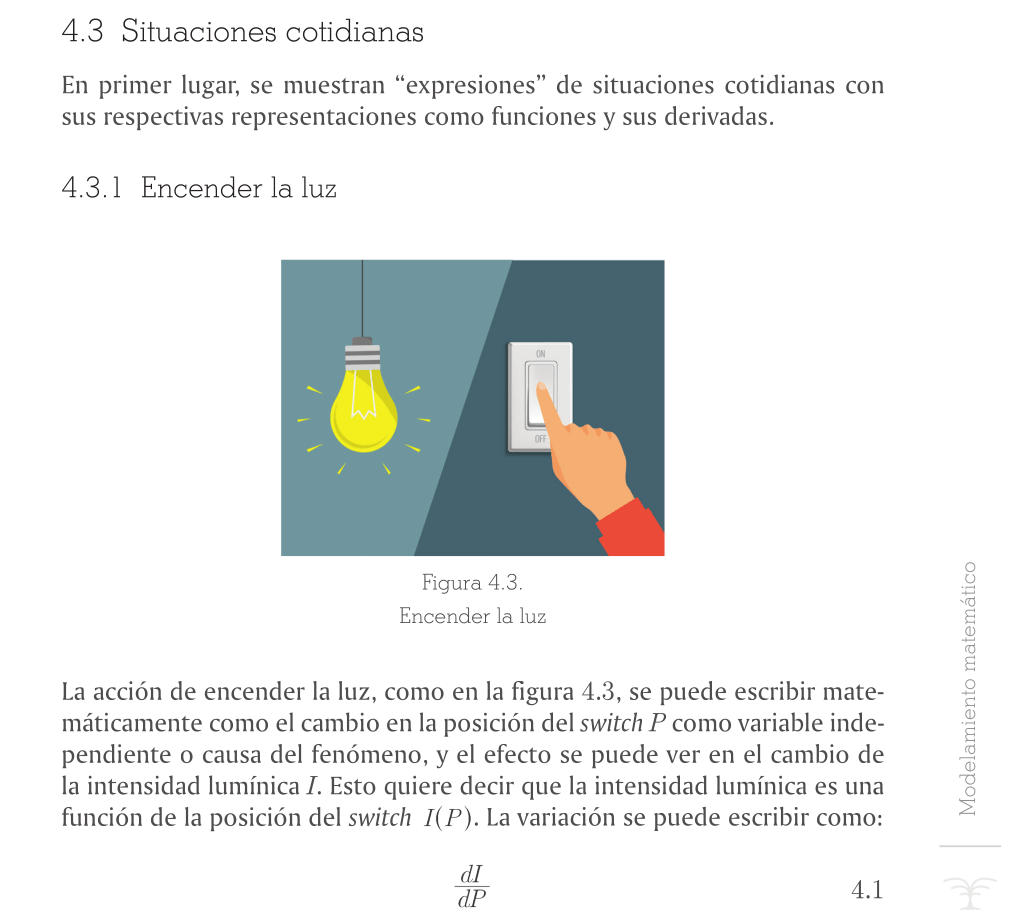
\includegraphics[height=7.4cm]{vida_cotidiana}
	\end{figure}
	\note{
		En la diapositiva se muestra una de estas situaciones diarias.

		También se tiene un anexo donde se estudia un software libre como
		es \lstinline|wxmaxima|.
	}
\end{frame}
\section{DUNE Numerics Project}

\begin{frame}
	\frametitle{\secname}

	\begin{alertblock}{Distributed and Unified Numerics Environment (DUNE)}
		\note{
			Título: ``Una introducción a la caja de herramientas Dune en
			C++/Python para la solución de modelos matemáticos''.

			Se hará una breve presentación de la caja de herramientas
			modular Dune Numerics, biblioteca modular desarrollada en la
			Universidad de Heildeberg en C++ y Python, para resolver
			ecuaciones diferenciales parciales utilizando métodos basados
			en mallas, por ejemplo, diferencias finitas, elementos finitos
			o volúmenes finitos.

			Es un software de código abierto bajo la licencia GNU General
			Public Licence 2, con binarios disponibles para las
			distribuciones Arch Linux en el repositorio arch4edu, Debian,
			openSUSE Tumbleweed y Ubuntu; también los scripts de
			compilación a través de Homebrew Formulae en macOS, los
			FreshPorts de FreeBSD y el Arch User Repository
			(AUR) en Arch Linux.

			Se mostrará la estructura general, algunos proyectos basados en
			Dune y algunas simulaciones de modelos matemáticos que incluyen
			este tipo de ecuaciones y sus respectivas soluciones, así como
			una implementación breve de Dune Numerics.
		}
		\begin{itemize}
			\item

			      Software de \alert{código abierto} bajo la licencia GNU
			      General Public Licence 2~\gpllicense{}.

			\item

			      Disponible en
			      \href{https://github.com/dune-copasi/homebrew-tap}{macOS},
			      \href{https://packages.debian.org/search?suite=sid&section=all&arch=any&searchon=sourcenames&keywords=dune-}{Debian}~\debian{},
			      \href{https://launchpad.net/~opm/+archive/ubuntu/ppa}{Ubuntu}~\ubuntu{},
			      \href{https://build.opensuse.org/search?search_text=dune-&search_for=2&name=1&attrib_type_id=}{openSUSE}~\opensuse{},
			      \href{https://aur.archlinux.org/packages/?O=0&SeB=n&K=dune-&outdated=&SB=n&SO=a&PP=50&do_Search=Ir}{\alert{Arch Linux}}~\archlinux{}
			      y \href{https://www.freshports.org/search.php?stype=name&method=match&query=dune-&num=20&orderby=category&orderbyupdown=asc&search=Search&format=html&branch=head}{FreeBSD}~\freebsd{}.

			\item

			      Conjunto de \alert{bibliotecas de plantillas}
			      en~\cpplogo{} moderno con enlaces
			      a~\href{https://pypi.org/search/?q=dune-}{\pythonlogo{}}.

			      \note{
				      Desarrollado con CMake, escrito en C++ moderno
				      con enlaces Python a través de \texttt{pybind11}.
			      }

			\item

			      \alert{Implementación eficiente} de las estructuras
			      de datos y los algoritmos en interfaces abstractas.

			\item

			      Para la resolución numérica de
			      \alert{ecuaciones diferenciales parciales} e
			      implementación de esquemas basados en mallas, por
			      ejemplo, \emph{diferencias finitas},
			      \emph{elementos finitos} o
			      \emph{volúmenes finitos}.
		\end{itemize}
	\end{alertblock}

	\begin{minipage}{0.45\textwidth}
		\begin{figure}[ht!]
			\centering
			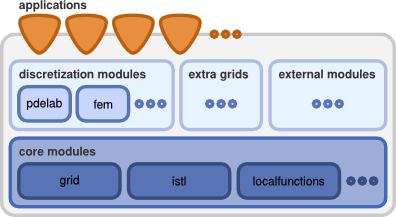
\includegraphics[height=3.2cm]{dunedesign}
			\caption*{
				\textbf{Origen:}~\url{https://dune-project.org/about/dune}.
			}
		\end{figure}
	\end{minipage}\qquad\qquad
	\begin{minipage}{0.45\textwidth}
		\begin{figure}[ht!]
			\centering
			\href{https://github.com/arch4edu/arch4edu}{
\includegraphics[height=2.8cm]{arch4edu}}\quad\quad
			\href{https://github.com/arch4edu/cactus}{
\includegraphics[height=2.8cm]{cactus}}
			\caption{Los binarios están disponible en el repositorio
				\alert{Arch Linux for Education}
				(Jingbei Li, Carlos Aznarán y otros, octubre 2022).
			}
		\end{figure}
	\end{minipage}
	\note{
		The easiest way to install the binaries are from Arch Linux
		Repository for Education.
		Jingbei Li, Carlos Aznarán, et al.
	}
\end{frame}

\begin{frame}
	\frametitle{\secname}
	\framesubtitle{\subsecname}

	\begin{columns}
		\begin{column}{0.4\textwidth}
			\begin{alertblock}{Proyectos que emplean DUNE}

				\

				\begin{itemize}
					\item

					      \url{https://dumux.org}

					      \

					\item

					      \url{https://opm-project.org}

					      \

					\item

					      \url{https://precice.org}

					      \

					\item

					      \url{https://amdis.readthedocs.io}

					      \

					\item

					      \url{https://github.com/parafields}

					      \

					\item

					      \url{https://www.zib.de/projects/kaskade7-finite-element-toolbox}
				\end{itemize}
			\end{alertblock}
		\end{column}

		\begin{column}{0.6\textwidth}
			\begin{figure}[ht!]
				\centering
				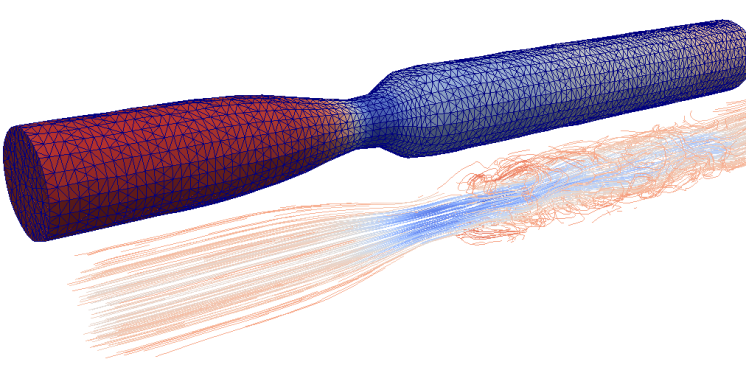
\includegraphics[width=6.05cm]{blood_girke}
				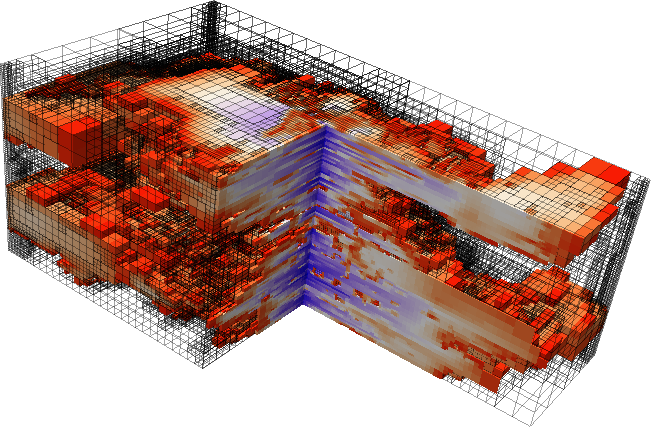
\includegraphics[width=6.05cm]{SPE10-benchmark}
				\caption*{\textbf{Origen:}~\url{https://dune-project.org/gallery}.}
			\end{figure}
		\end{column}
	\end{columns}
	\note{
		Presento las tres primeras páginas, la última versión estable de
		Dune es 2.8.0, pero la versión 2.9.0 se lanzó en octubre del
		2022.

		DuMu\textsuperscript{x} es un simulador con modelos multifásicos
		de varias componentes, geomecánica, redes de poros,
		problemas de almacenamiento de gases, ley de Fick, Darcy,
		Richards, etc.

		El módulo opm-flow se puede apoyar del visualizador de simulación
		llamado \emph{Resinsight}.
	}
\end{frame}
\section{El DUNE verso: módulos}

\begin{frame}[fragile]
	\frametitle{\secname}
	\framesubtitle{\url{https://dune-project.org/groups/core}}

	\begin{figure}[ht!]
		\centering
		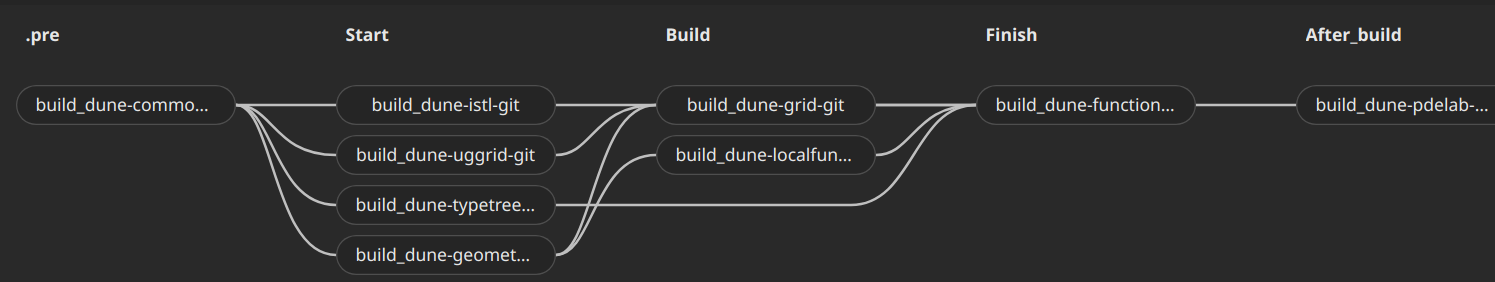
\includegraphics[width=14.6cm]{dependences}
		\caption{Tomado de \url{https://gitlab.com/dune-archiso/repository/dune-archiso-repository-pdelab-git/-/pipelines}}
	\end{figure}

	\begin{description}
		\item[dune-common]

			Clases fundamentales e infraestructura para la construcción del sistema.

		\item[dune-geometry]

			Elementos de referencia, métodos de cuadratura y transformaciones geométricas.

		\item[dune-grid]

			Interfaces con las mallas (ALUGrid, UGGrid, Alberta, YasGrid), construcción y visualización.

		\item[dune-istl]

			Biblioteca de solucionadores iterativas de plantillas, clases genéricas de matrices/vectores dispersos, solucionadores

		\item[dune-localfunctions]

			Interface genérica para funciones de elementos finitos.
	\end{description}

	\note{
		\begin{description}
			\item[dune-common]
				Contiene las clases base usadas por todos los módulos de DUNE-modules.

				Provee algunas clases de infraestructura para depuración y manejo de excepciones así como una librería para manejar una matriz densa y vectores.

			\item[dune-grid]
				Define mallas jerarquizadas, paralelas, de dimensiones arbitrarias, permite salida a formatos que puedens ser leídos por ParaView.
		\end{description}
	}
\end{frame}

\subsection{Dependencias de algunos módulos}

\begin{frame}
	\frametitle{\secname}
	\framesubtitle{\subsecname}

	\begin{columns}
		\begin{column}{0.5\textwidth}
			\dirtree{%
				.1 dune-fem.
				.2 dune-grid.
				.3 dune-geometry.
				.4 dune-common.
			}

			\

			\

			\dirtree{%
				.1 dumux.
				.2 dune-istl.
				.2 dune-localfunctions.
				.2 vc.
				.2 psurface.
				.2 superlu.
				.2 arpack++.
				.2 suitesparse.
				.2 dune-alugrid.
				.2 dune-subgrid.
				.2 fmt.
				.2 opm-common.
			}
		\end{column}

		\begin{column}{0.5\textwidth}
			\dirtree{%
				.1 opm-upscaling.
				.2 opm-grid.
				.3 opm-common.
				.4 dune-grid.
				.5 dune-geometry.
				.4 dune-istl.
				.4 boost.
			}

			\

			\

			\dirtree{%
				.1 opm-models.
				.2 opm-material.
				.3 opm-common.
				.4 dune-grid.
				.5 dune-geometry.
				.4 dune-istl.
				.4 boost.
			}
		\end{column}
	\end{columns}

	\note{
		Aquí se puede ver la relación de dependencias entre los módulos de DUNE.
	}

\end{frame}
\section{Curso de DUNE/PDELab $2021$}

\begin{frame}[fragile]
	\frametitle{\secname}
	\framesubtitle{\url{https://dune-pdelab-course.readthedocs.io}}

	\begin{figure}[ht!]
		\centering
		\href{https://dune-pdelab-course.readthedocs.io}{
			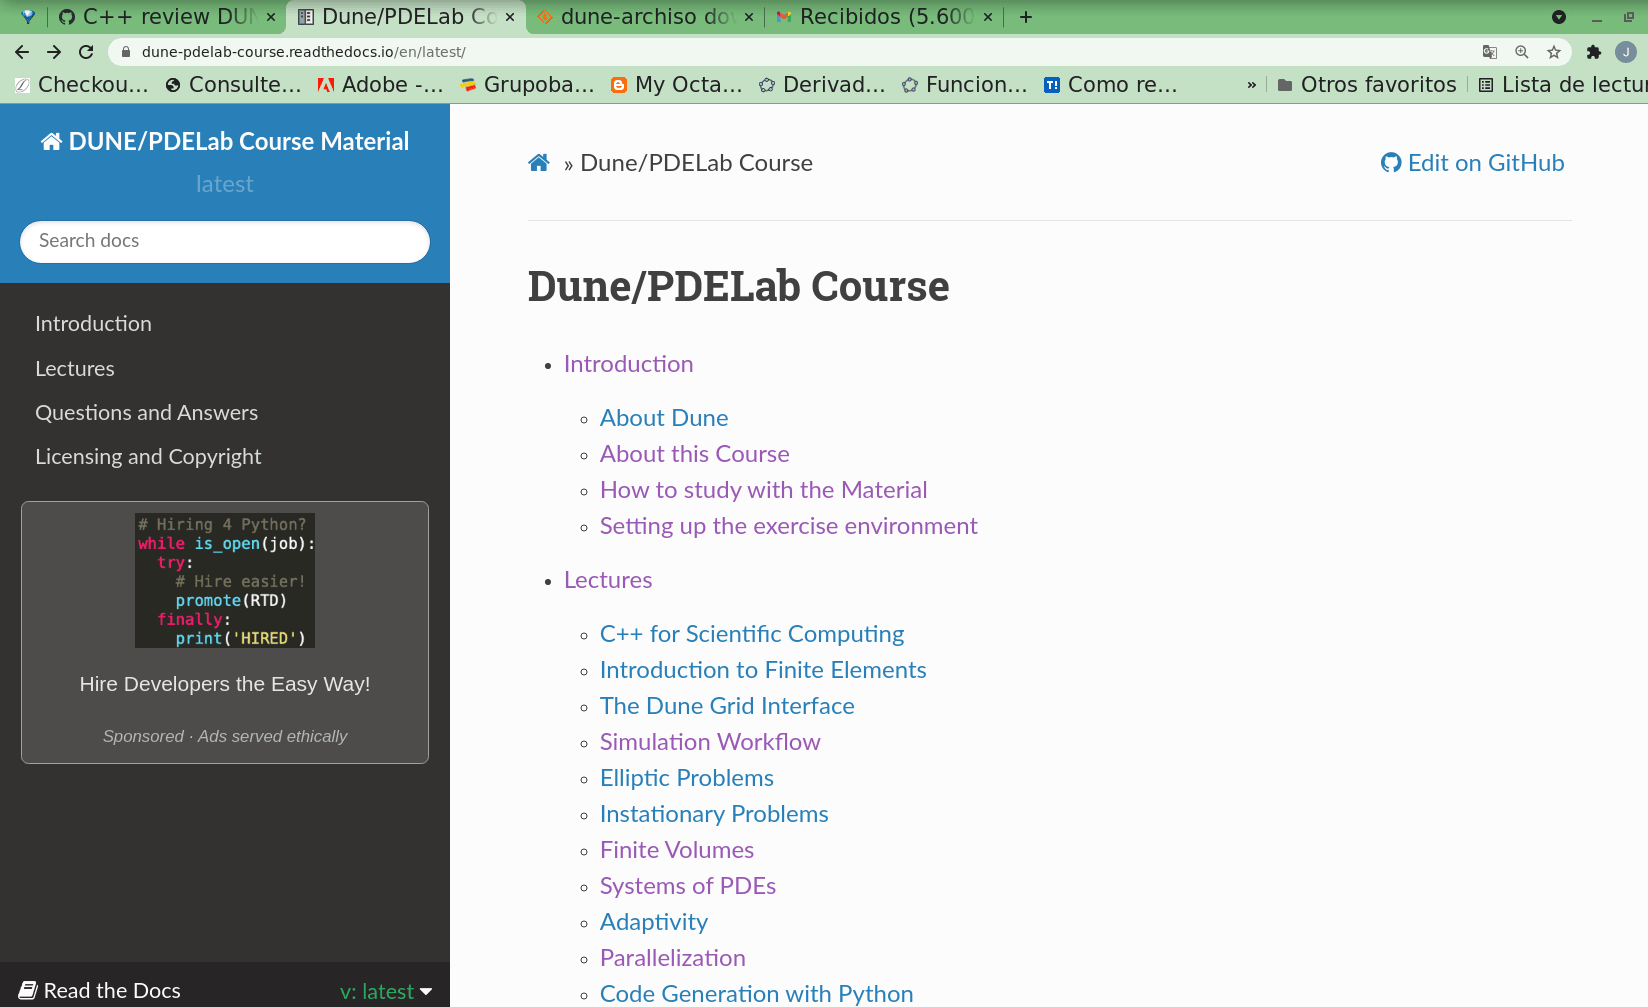
\includegraphics[height=7.3cm]{dune_course_2021}}
	\end{figure}
	\note{
		Cursos de DUNE anuales, lista de correo de preguntas y noticias.

		Cuenta con nueve tutoriales.
		El módulo se llama dune-pdelab-tutorials,
		\url{https://gitlab.dune-project.org/pdelab/dune-pdelab-tutorials},
		es el sucesor de dune-grid-howto
		\url{https://gitlab.dune-project.org/core/dune-grid-howto}.
	}
\end{frame}

\begin{frame}[fragile]
	\frametitle{Snippet en C++}
	\footnotesize
	\lstinputlisting[
		caption={Programa \texttt{dune-basics.cc}.},
		label=dune-basics.cc
	]{dune-basics.cc}
	\note{
		Se muestra un código minimo de un programa basado en Dune.
		La forma de trabajo es importar las clases con las directivas
		% \lstinline|#include <dune/modulo/cabecera.hh>|

		\url{https://www.dune-project.org/sphinx/content/sphinx/dune-fem/mcf_nb.html}
		Es una simulación dinámica.
	}
\end{frame}

{
\usebackgroundtemplate{
	\centering
	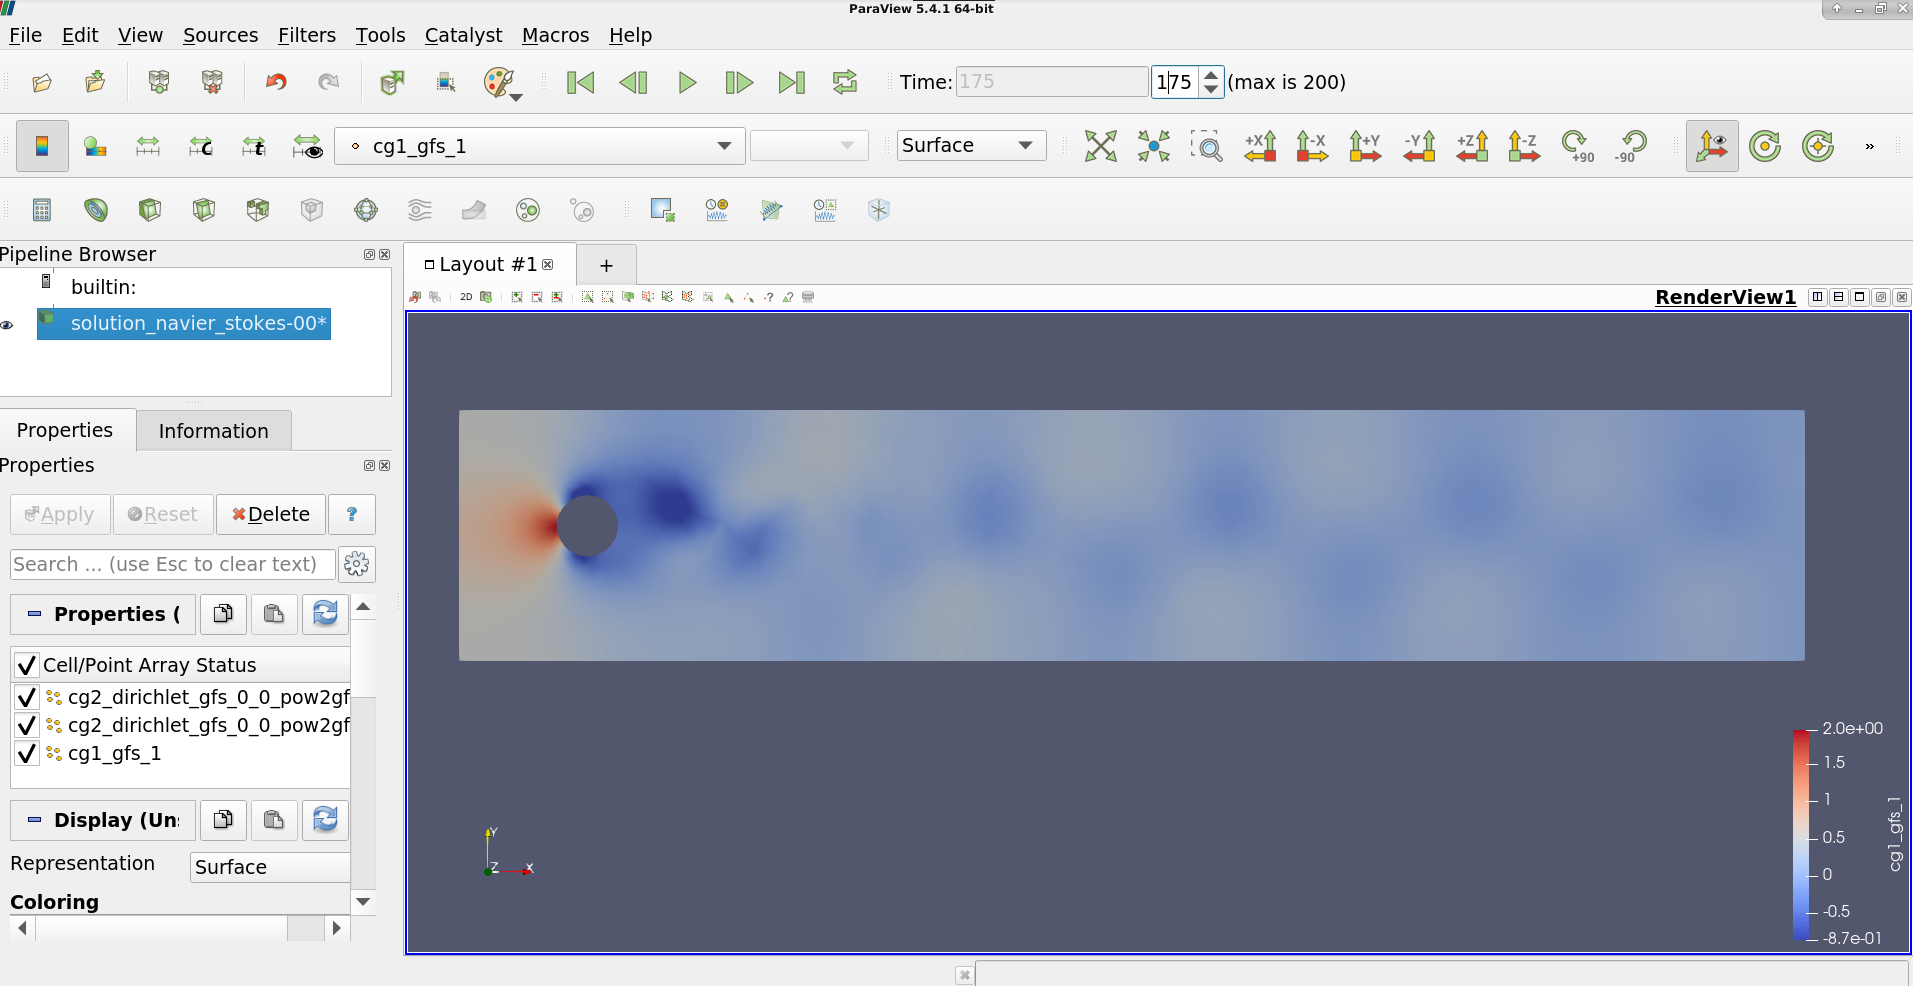
\includegraphics[width=\paperwidth]{tutorial-9}
}

\begin{frame}[plain]
	\note{
		Presentar el vídeo presenta la simulación de un flujo que
		obedece las ecuaciones de Navier Stokes, alrededor de un
		cilindro.
	}
\end{frame}
}

\begin{frame}[fragile]
	\frametitle{Snippet en Python}
	\framesubtitle{\url{https://dune-project.org/sphinx/content/sphinx/dune-fem}}
	\begin{figure}[ht!]
		\centering
		\href{https://www.dune-project.org/sphinx/content/sphinx/dune-fem/mcf_nb.html}{
			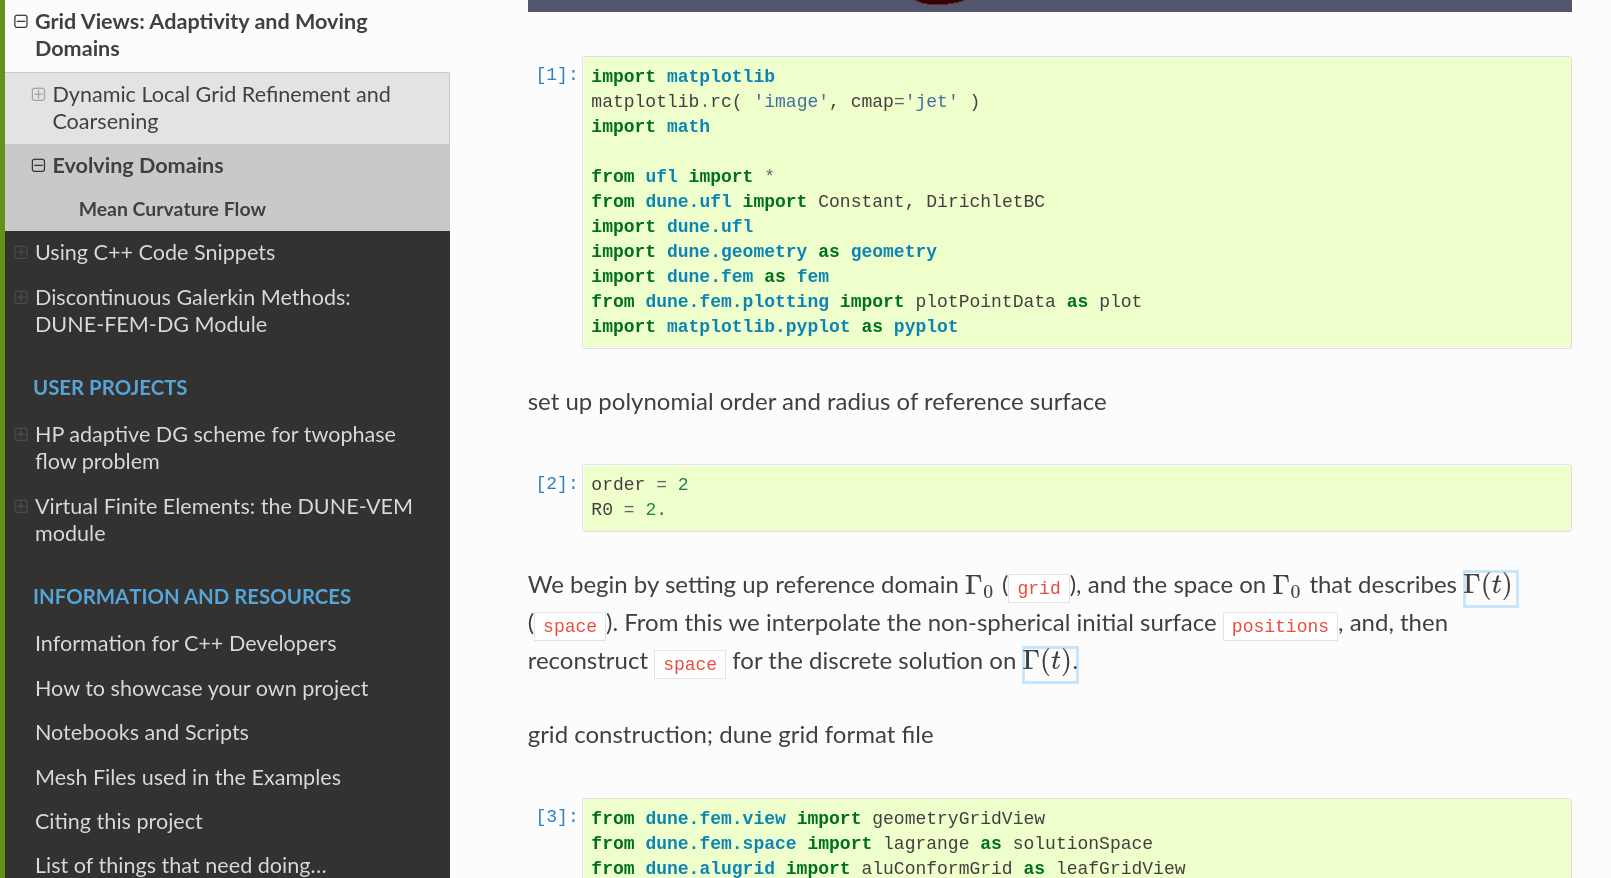
\includegraphics[height=7.3cm]{python_code}}
	\end{figure}

\end{frame}

{
\usebackgroundtemplate{\centering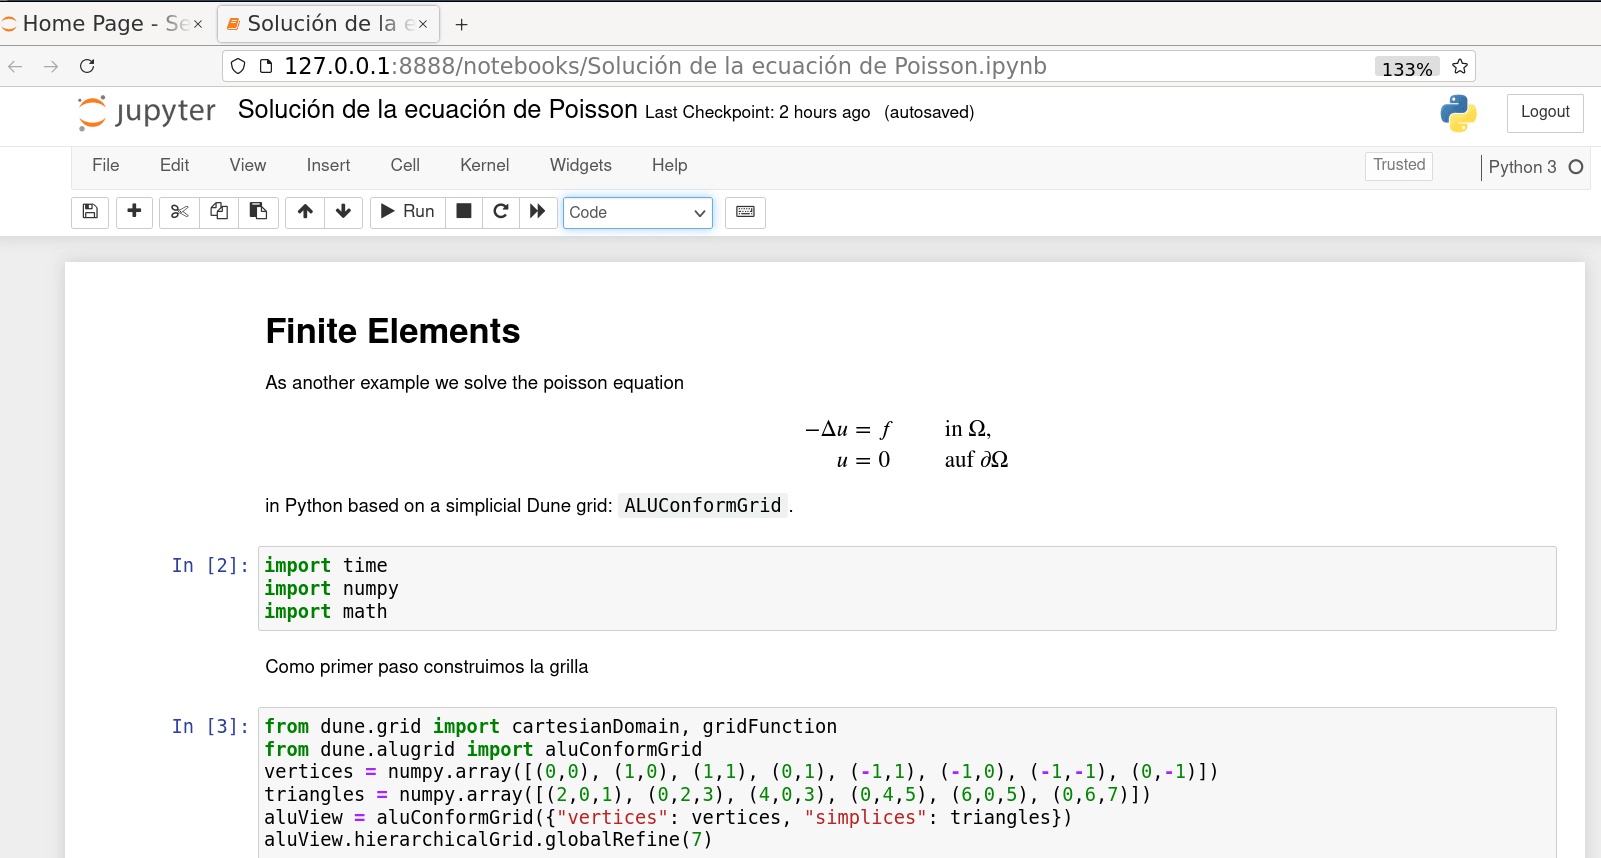
\includegraphics[width=\paperwidth]{jupyter01}}
\begin{frame}[plain]
	\note{
		Mostrar el artículo de dune-python
		\url{https://arxiv.org/abs/1807.05252}, página 11.
		Los bindings de dune se encuentran en cada módulo, por ejemplo,
		dune-common, dune-geometry, dune-grid, dune-istl, etc, que
		depende de la instalación en C++ de dicho módulo.
	}
\end{frame}
}

{
\usebackgroundtemplate{\centering\href{https://github.com/cpp-review-dune}{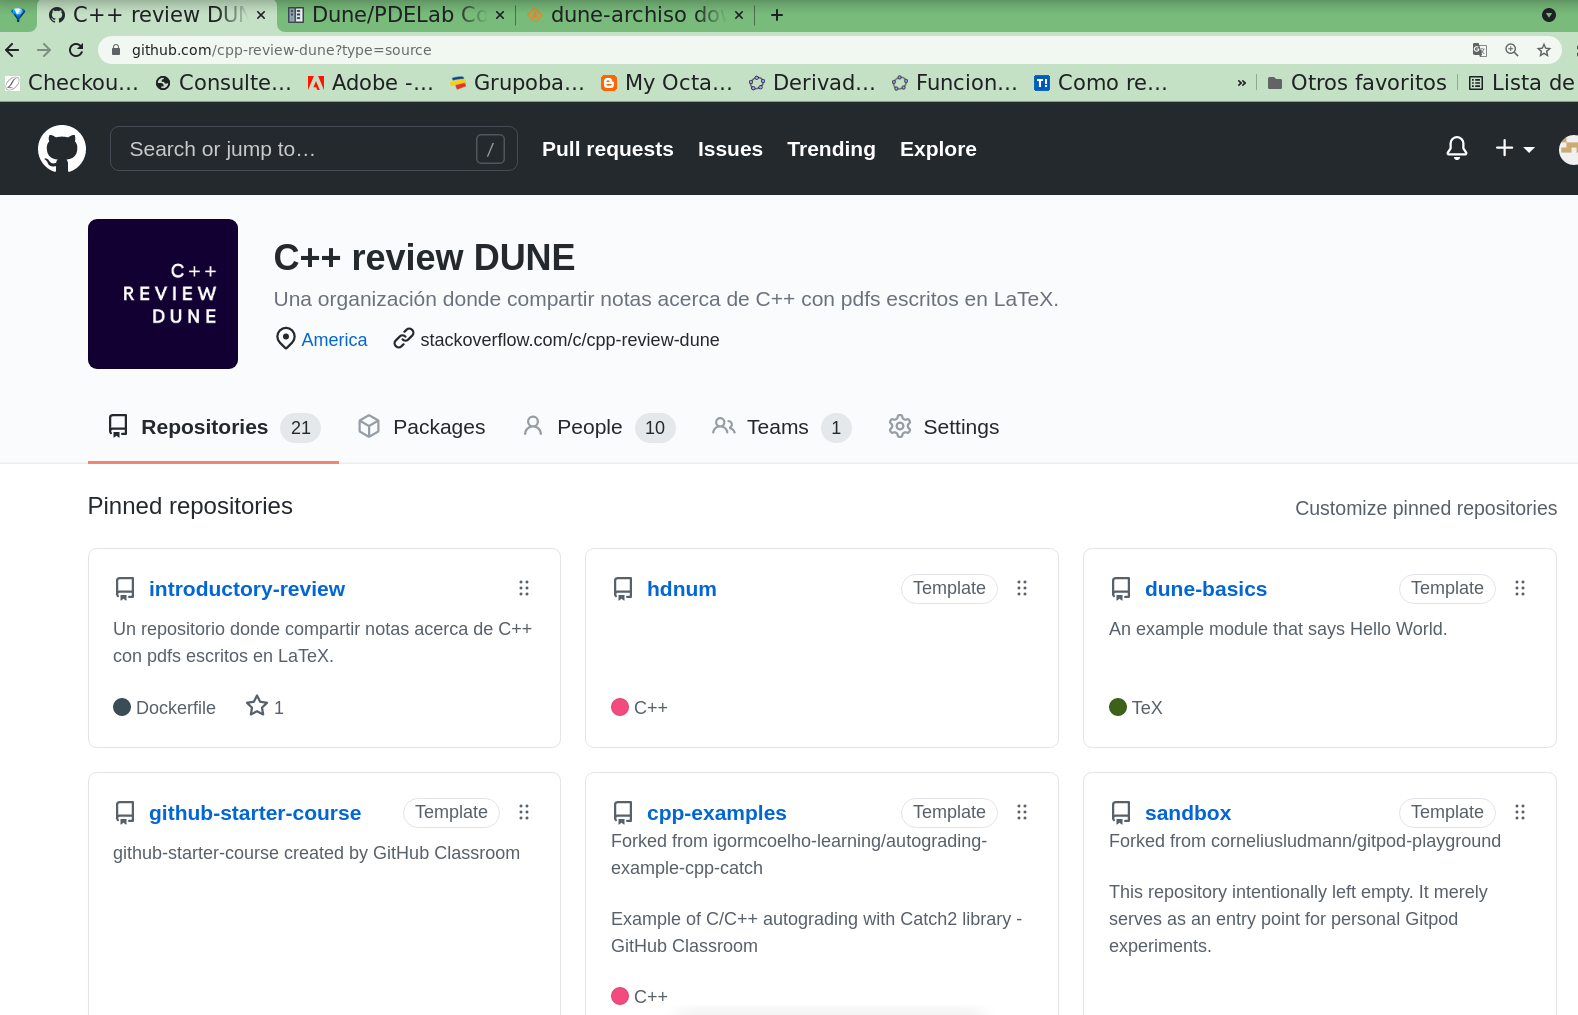
\includegraphics[width=\paperwidth]{cpp_review}}}
\begin{frame}[plain]
	\note{
		Página para repasar el curso virtual de DUNE/PDELab en el que
		contamos con los siguientes repositorios:

		\begin{itemize}
			\item

			      \url{https://cpp-review-dune.github.io/introductory-review}
			      que contiene enlaces de interés y el enlace de acceso al
			      grupo de Telegram.
			      Además de otros cursos relacionados.
			      Vídeos.

			\item

			      Portar diversos módulos de DUNE en Arch Linux (listo).

			\item

			      La creación de imágenes Docker que permite la utilización
			      de módulos específicos, incluidos la versión de Python,
			      de manera periódica y automática, esto se puede ver en la
			      sección de Actions en el repositorio introductory-review.

			\item

			      Por otro lado, han estado adoptando la metodología de Git
			      en un proyecto de la Universidad Nacional de Colombia.
		\end{itemize}
	}
\end{frame}
}


{
	\usebackgroundtemplate{\centering\href{https://github.com/cpp-review-dune}{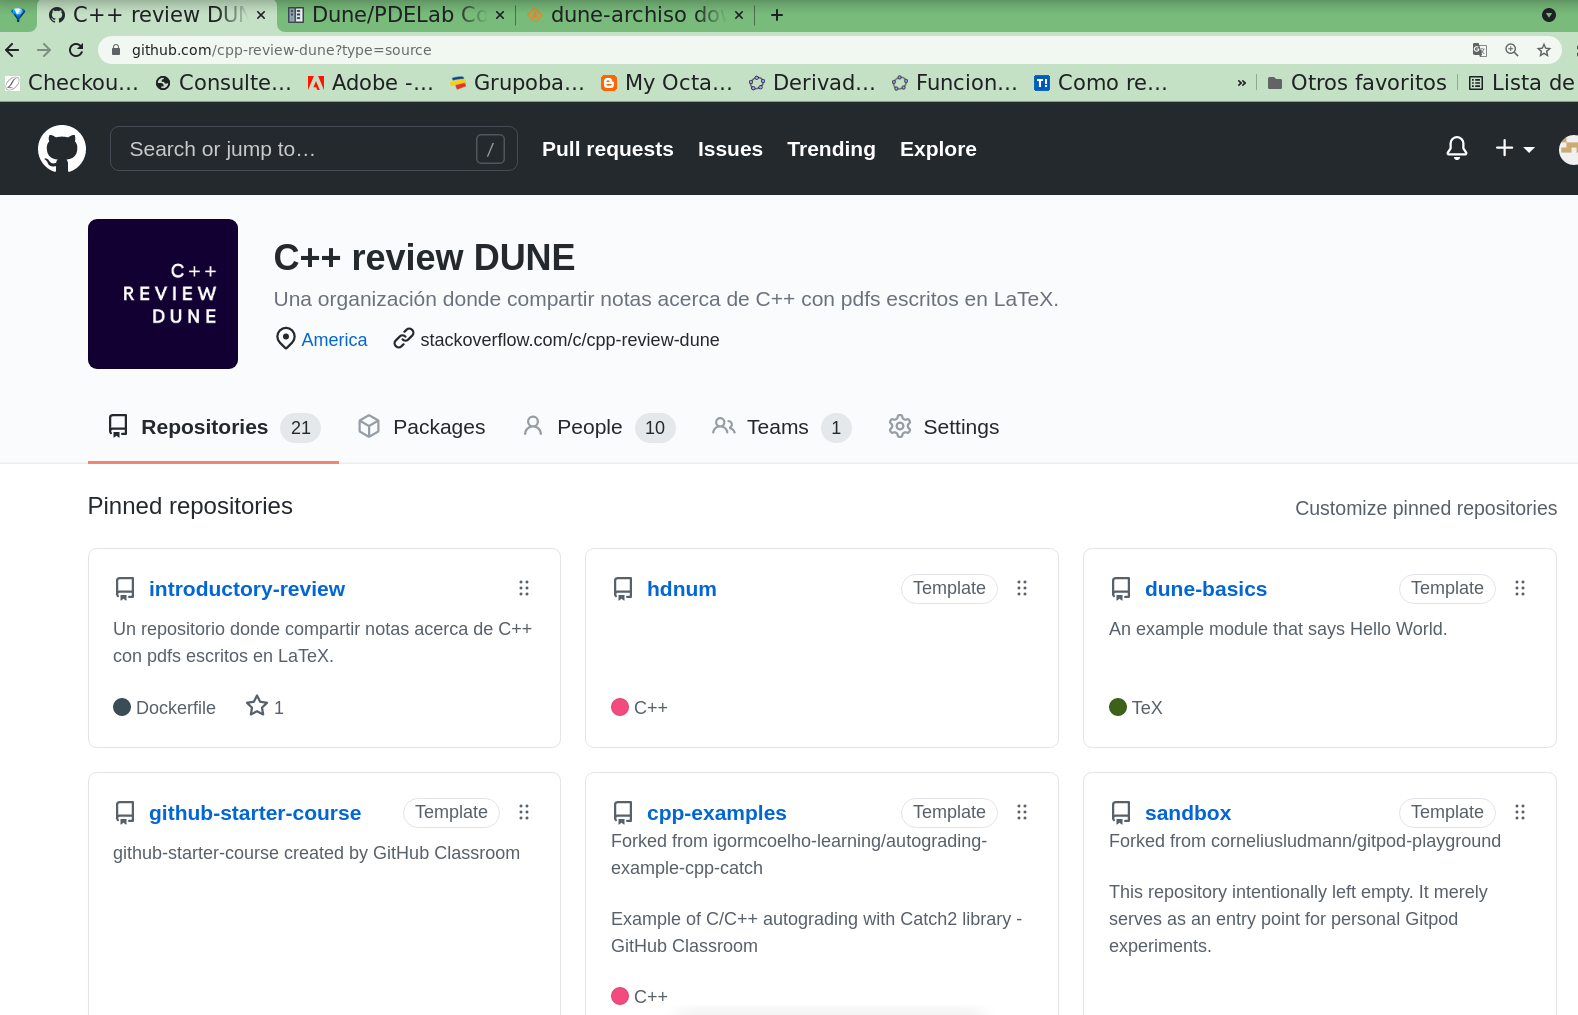
\includegraphics[width=\paperwidth]{cpp_review}}}
	\begin{frame}[plain]
		\note{
			Página para repasar el curso virtual de DUNE/PDELab en el que contamos con los siguientes repositorios:
			\begin{itemize}
				\item \url{https://cpp-review-dune.github.io/introductory-review}
				      que contiene enlaces de interés y el enlace de acceso al grupo de Telegram. Además de otros cursos relacionados. Vídeos.
				\item Portar diversos módulos de DUNE en Arch Linux.
				\item La creación de imágenes Docker que permite la utilización de módulos específicos, incluidos la versión de Python, de manera periódica y automática, esto se puede ver en la sección de Actions en el repositorio introductory-review
				\item Por otro lado, han estado adoptando la metodología de Git en un proyecto de la Universidad Nacional de Colombia.
			\end{itemize}
		}
	\end{frame}
}

{
	\usebackgroundtemplate{\centering\href{https://sourceforge.net/projects/dune-archiso}{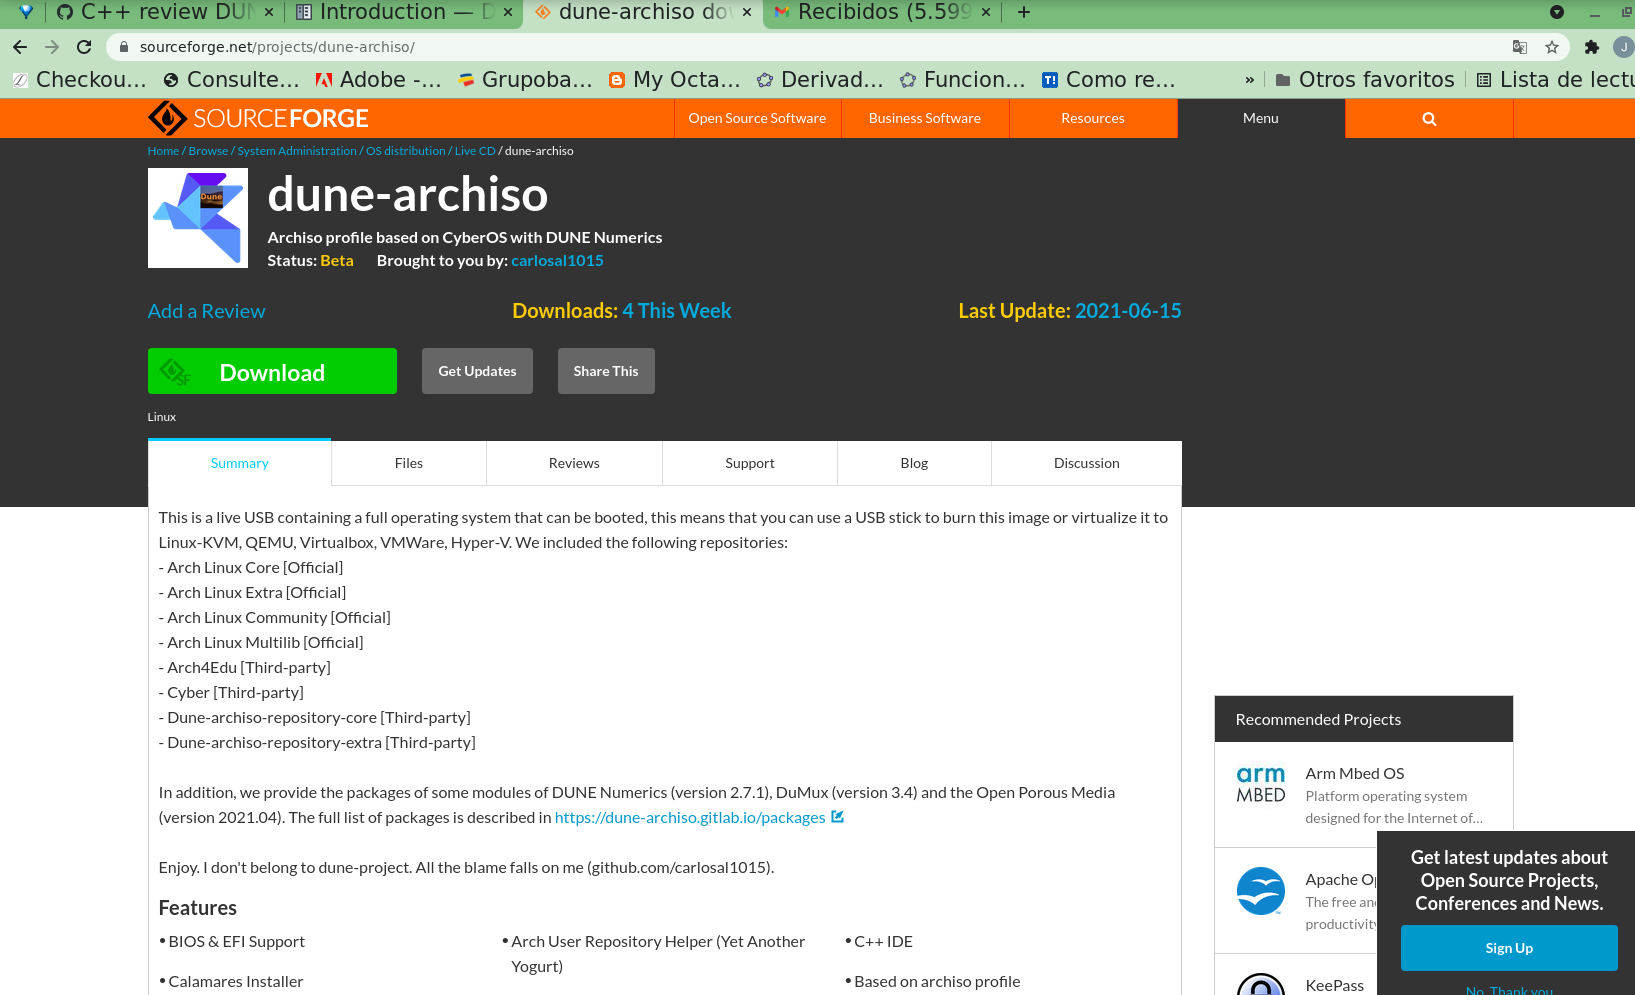
\includegraphics[width=\paperwidth]{archiso}}}
	\begin{frame}[plain]
	\end{frame}
}

\begin{frame}\transblindsvertical
	\frametitle{Referencias}
	\only<1>{
		\begin{itemize}
			\item

			      Libros

			      \

			      \nocite{*}
			      \printbibliography[heading=none,keyword=book]
		\end{itemize}
	}

	\

	\only<2>{
		\begin{itemize}
			\item

			      Artículos

			      \

			      \printbibliography[heading=none,keyword=paper]
		\end{itemize}
	}
\end{frame}

\begin{frame}\transblindsvertical
	\frametitle{Referencias}
	\begin{itemize}
		\item

		      Sitios web

		      \

		      \printbibliography[heading=none,keyword=online]
	\end{itemize}
\end{frame}
\begin{frame}
	\frametitle{Agradecimientos}
	\begin{center}\LARGE
		¡Muchas gracias!
	\end{center}
	\begin{figure}[ht!]
		\centering
		
\includegraphics[height=1.4cm]{alfaomega}\quad
		
\includegraphics[height=1.9cm]{unal}\quad
		
\includegraphics[height=1.6cm]{dune-logo}
	\end{figure}
	\vfill
	\begin{minipage}{0.75\paperwidth}
		\textcolor{c++reviewduneblue}{Presentación disponible en:}
		\begin{center}
			\href{https://github.comhttps://github.comhttps://github.com}{\url{https://github.comhttps://github.comhttps://github.com}}
		\end{center}
	\end{minipage}
	\hfill
	\begin{minipage}{0.25\paperwidth}
		\begin{flushright}
			Dudas, sugerencias o preguntas a:

			\

			\href{mailto:jlealgom@unal.edu.co}{jlealgom\MVAt unal.edu.co}

			\href{mailto:caznaranl@uni.pe}{caznaranl\MVAt uni.pe}
		\end{flushright}
	\end{minipage}

\end{frame}

\end{document}